\documentclass{article}
\usepackage[latin1]{inputenc}    
\usepackage[T1]{fontenc}
\usepackage[french]{babel}
\usepackage{graphicx}
\newcommand\tab[1][1cm]{\hspace*{#1}}
\usepackage{geometry}
\geometry{hmargin=3.45cm,vmargin=3cm}
\usepackage{color}
\definecolor{myblue}{rgb}{0.15, 0.15, 0.8}

\begin{document}

\newpage
\title{Cahier des spécifications\\Sujet 10 : Réseau de Neurones}
\author{Thibaut \bsc{Pepin}\\Soumia \bsc{Rezgui}\\Isaac \bsc{Szulek}\\Severine \bsc{Selaquet}\\Anthony \bsc{Montigne}\\Arezki \bsc{Slimani}}
\maketitle

\newpage

\small{\tableofcontents}

\newpage
\section{Introduction}
 Nous souhaitons analyser des images, un problème compliqué qui a besoin de prendre en entrée une image et dont le but est d'essayer de deviner ce que représente cette image.
Pour cela il nous faut une structure qui sera capable de prendre beaucoup de données en entrée et de capturer des relations complexes entres les entrées et les sorties,c'est là qu'interviennent les réseaux de neurones artificiels.
Ainsi, afin d'indiquer comment réaliser le besoin defini par le cahier des charges, il est necessaire de reprendre les besoins du maitre d'ouvrage, en les exprimant cette fois par les maîtres d'oeuvres.
En ce sens , nous avons donc réaliser une description détaillée pour notre conception technique. Le document suivant est ainsi la définition écrite, en terme de fonctionalité et de performance, du cahier des charges préalablement établis.

\section{Structures de Données}
	\subsection{Réseau de neurones}
	Pour le choix de notre structure de données nous avons rapidement adopté la représentation d'un réseau de neurones comme un ensemble de couches et non comme un ensemble de neurones individuels. 
	Chaque couche doit donc contenir l'ensemble des activations, des biais et des poids des neurones de cette couche.
	On stocke les activations et les biais dans des vecteurs et les poids dans des matrices.
	Nous les avons integré dans une structure couche comme tableau à une ou deux dimensions (car les calculs a effectuer necessite d'accéder aux éléments sans ordre particulier).	
	Afin de stocker l'ensemble des couches constituant le réseau de neurone, nous avons opté pour une liste doublement chainée. 
	En effet, les deux algorithmes necessitant d'accéder aux contenus des couches vont propager des informations de la premiere couche à la dernière couche pour l'algorithme de propagation. 
	Et de la dernière couche à la première couche pour l'algorithme de rétro-propagation (d'où le double chainage).	
	Afin de regrouper les informations générales d'un réseau de neurones, nous avons crée une petite structure contenant toutes sortes d'informations comme la date de création.	
	Un réseau de neurones est donc constitué d'une structure d'informations ainsi que d'un pointeur sur la premiere couche et d'un autre pointeur sur la dernière couche.

	\begin{flushleft}
	
		struct COUCHE	//structure représentant une couche (ensemble de neurones) dans un réseau de neurone\\
		\{\\
			\tab \textcolor{myblue}{\textbf{float*}} A;	//tableau représentant le vecteur des activation des neurones d'une couche. Possède autant d'élements que de neurones présent dans la couche.\\
			\tab \textcolor{myblue}{\textbf{float*}} B;	//tableau représentant le vecteur des biais des neurones d'une couche de même taille que le tableau A.\\
			\tab \textcolor{myblue}{\textbf{float**}} W;	//tableau à deux dimensions représentant la matrice des poids entre les neurones de la couche précedente et les neurones de cette couche. Ce tableau est donc de taille (taille de la couche actuelle * taille de la couche précedente) et est composé d'élements $w_{ij}$ où j est le numéro du neurone de la couche précedente et i le numéro du neurone de la couche actuelle.\\
			\tab \textcolor{myblue}{\textbf{int}} taille;	//Indique le nombre de neurones présent dans cette couche\\
			\tab \textcolor{myblue}{\textbf{float}} DELTA;      //tableau représentant le vecteur des modifications à apporter aux biais de cette couche lors de la rétro-propagation des neurones d'une couche de même taille que le tableau A.\\
			\tab \textcolor{myblue}{\textbf{float**}} DELTA\_M; //tableau à deux dimensions représentant la matrice des modifications à apporter aux poids de cette couche lors de la rétro-propagation des neurones d'une couche de même taille que la matrice W\\
			\medbreak
			\tab \textcolor{myblue}{\textbf{struct COUCHE*}} prec;	//pointeur sur la couche précédente.\\
			\tab \textcolor{myblue}{\textbf{struct COUCHE*}} suiv;	//pointeur sur la couche suivante.\\
		\};\\
		\bigbreak
		typedef struct COUCHE COUCHE;\\
		typedef COUCHE* Liste\_couche;\\
		\bigbreak
		struct INFO\_RN	//structure représentant les différentes informations caractérisant un réseau de neurones.\\
		\{\\
			\tab \textcolor{myblue}{\textbf{char**}} etiquettes;	//tableau de chaine de caractère comprenant la signification des neurones de sortie.\\
			\tab \textcolor{myblue}{\textbf{char*}} nom;	//nom donné au réseau de neurones.\\
			\tab \textcolor{myblue}{\textbf{char*}} date;	//date de création du réseau de neurones.\\
			\tab \textcolor{myblue}{\textbf{int}} reussite;	//nombre de fois ou le réseau de neurones a obtnenu la réponse attendue lors de l'apprentissage.\\
			\tab \textcolor{myblue}{\textbf{int}} echec;	//nombre de fois ou le réseau de neurones n'a pas obtnenu la réponse attendue lors de l'apprentissage.\\
		\};\\
		\bigbreak
		typedef struct INFO\_RN INFO\_RN;\\
		\bigbreak
		struct RN	//structure représentant le réseau de neurones, contenant l'ensemble des couches et les informations du réseau de neurones.\\
		\{\\
			\tab \textcolor{myblue}{\textbf{INFO\_RN}} info;	//les informations du réseau de neurones.\\
			\tab \textcolor{myblue}{\textbf{Liste\_couche}} couche\_deb;	//pointeur sur la 1ère couche du RN.\\
			\tab \textcolor{myblue}{\textbf{Liste\_couche}} couche\_fin;    //pointeur sur la dernière couche du RN.\\
		\};\\
		\bigbreak
		typedef struct RN RN;
		
	\end{flushleft}
	
	\subsection{Image}
	Afin de représenter une image, nous avons opté pour un tableau à une dimension de pixel afin de se rapprocher de la structure des vecteurs d'activations.
	Chaque pixel étant une structure contenant la quantité de rouge, de vert et de bleu présent dans un nombre entre 0 et 255 d'où le type char qui convient parfaitement pour des valeurs dans cet intervalle.
	\begin{flushleft}
		typedef struct Pixel\\
			\{\\
				\tab \textcolor{myblue}{\textbf{unsigned char}} r,g,b;\\
			\} Pixel;
		\bigbreak
		typedef struct Image\\
			\{\\
				\tab \textcolor{myblue}{\textbf{int}} w,h;\\
				\tab \textcolor{myblue}{\textbf{Pixel*}} dat;\\
			\} Image;
	\end{flushleft}
	
	\subsection{Apprentissage}
	Le couple d'information sortie attendue et donnée d'entrée étant nécessaire lors de l'apprentissage. Nous les avons regroupé dans une petite structure.
	\begin{flushleft}
		typedef struct Apprentissage\\
			\{\\
				\tab \textcolor{myblue}{\textbf{Image*}} image;\\
				\tab \textcolor{myblue}{\textbf{char*}} etiquette;\\
			\} App;
	\end{flushleft}
	
	\newpage
	
	
	
	
	
	
\section{Signatures des Fonctions}
	\subsection{Gestionnaires d'apprentissage}
			\subsubsection{\textcolor{myblue}{\textbf{void}} BackProp(\textcolor{myblue}{\textbf{RN*}}, \textcolor{myblue}{\textbf{App*}}, \textcolor{myblue}{\textbf{float}})}
				Backprop va effectuer l'algorithme de propagation-inverse puis va modifier les poids et les biais du réseau de neurones passé en paramètre.
				Pour cela il est nécessaire d'avoir le couple donnée d'entrée et sortie attendue présent ici dans la structure App*, on effectuera donc la propagation sur l'image et on comparera l'étiquette de sortie avec le char* qui est l'étiquette attendue.
				
			\subsubsection{\textcolor{myblue}{\textbf{void}} SigmoidePrimeZ(\textcolor{myblue}{\textbf{float*}} in, \textcolor{myblue}{\textbf{float**}} out, \textcolor{myblue}{\textbf{int}} taille)}
			SigmoidePrimeZ va récupérer les éléments stockés dans le premier tableau contenant 'taille' éléments puis effectuer l'opération $x*(1-x)$ sur chaque éléments avant de les écrire dans le deuxième tableau passé en paramètre. Cette opération n'est pas la dérivée de la fonction sigmoide, il s'agit d'une petite optimisation qui nous permet de trouver le même résultat plus rapidement. En effet lors de la propagation inverse il nous est necessaire d'effectuer l'opération : \\$\sigma'(z) = \sigma(z)*(1-\sigma(z))$\\ ou z vient de : \\$a^L = \sigma(w^L*a^{L-1}+b^L) = \sigma(z^L)$\\ or z n'est pas stocké dans notre structure et on peut de toute facon simplifier par :\\$\sigma'(z)=a*(1-a)$\\ d'ou cette fonction.\\
			Le deuxième tableau est a deux dimension car DELTA\_M est disponible au moment ou cette opération est effectuée, on va donc l'utiliser plutôt que de créer un autre tableau pour stocker le résultat.
			
			\subsubsection{\textcolor{myblue}{\textbf{void}} MultiplicationMatricielleTransposeeTM(\textcolor{myblue}{\textbf{float**}},  \textcolor{myblue}{\textbf{float*}},  \textcolor{myblue}{\textbf{float*}},  \textcolor{myblue}{\textbf{int}},  \textcolor{myblue}{\textbf{int}})\\
			\textcolor{myblue}{\textbf{void}} MultiplicationMatricielleTransposeeMT(\textcolor{myblue}{\textbf{float*}},  \textcolor{myblue}{\textbf{float*}},  \textcolor{myblue}{\textbf{float**}},  \textcolor{myblue}{\textbf{int}},  \textcolor{myblue}{\textbf{int}})}
				Lors de la retro-propagation certaines matrices doivent être transposées, ce qui est pénible à effectuer. Cependant, ces matrices transposées sont toujours multipliées par une autre matrice ce qui nous donne deux cas possibles : \\$A^T*B$ ou $B*A^T$\\MultiplicationMatricielleTransposeeTM et MultiplicationMatricielleTransposeeMT représentent ces deux cas mais ne transposent pas de matrice, elle effectue un produit matricielle où les matrices ne sont pas lues dans le sens conventionnel du produit matriciel afin d'obtenir le même résultat.
				
			\subsubsection{\textcolor{myblue}{\textbf{void}} Hadamard(\textcolor{myblue}{\textbf{float**}},  \textcolor{myblue}{\textbf{float*}},  \textcolor{myblue}{\textbf{float*}},  \textcolor{myblue}{\textbf{int}})}
				Hadamard effectue le produit vectoriel de Hadamard sur les deux premiers tableaux pour stocker le résultat dans le troisième tableau. Tous ces tableaux étant de même taille, celle ci est passée en paramètre.
				
			\subsubsection{\textcolor{myblue}{\textbf{void}} fct\_cout(\textcolor{myblue}{\textbf{RN}}, \textcolor{myblue}{\textbf{char*}})}
			 fct\_cout va calculer l'erreur entre le résultat obtenu lors de la propagation et le résultat attendu, soit le char*, pour chacun des neurones de la dernière couche du réseau de neurones puis va stocker le résultat dans le tableau DELTA de la dernière couche du réseau.
			
			\subsubsection{\textcolor{myblue}{\textbf{void}} ModifPoids(\textcolor{myblue}{\textbf{float**}},  \textcolor{myblue}{\textbf{float**}},  \textcolor{myblue}{\textbf{int}},  \textcolor{myblue}{\textbf{int}},  \textcolor{myblue}{\textbf{int}} eta)\\
			\textcolor{myblue}{\textbf{void}} ModifBiais(\textcolor{myblue}{\textbf{float*}},  \textcolor{myblue}{\textbf{float*}},  \textcolor{myblue}{\textbf{int}},  \textcolor{myblue}{\textbf{int}} eta)}
			ModifPoids et ModifBiais vont modifier le premier tableau passé en paramètre en lui soustrayant le deuxième tableau multiplié par la vitesse d'apprentissage 'eta', les autres paramètres sont les tailles des tableaux.
		
		
		
	\subsection{Gestionnaire d'entrées sorties}
		\subsubsection{\textcolor{myblue}{\textbf{Image*}} ChargerBmp(\textcolor{myblue}{\textbf{const char*}} fichier,  \textcolor{myblue}{\textbf{int}},  \textcolor{myblue}{\textbf{int}})\\
		\textcolor{myblue}{\textbf{Image*}} ChargerMnist(\textcolor{myblue}{\textbf{const char*}} fichier,  \textcolor{myblue}{\textbf{int}},  \textcolor{myblue}{\textbf{int}})}
		ChargerBmp et ChargerMnist vont lire à l'emplacement donné en paramètre et renvoyer le contenu du fichier sous forme de la structure Image, si celui ci contient une image au format bmp non compressé ou au même format que celui utilisé par la base de données MNIST.
		Le fichier est ensuite supprimé ou partiellement effacé.
		Les deux entiers correspondent à la largeur et la hauteur maximale de l'image acceptée par le réseau de neurones défini par l'utilisateur.
		
		\subsubsection{\textcolor{myblue}{\textbf{int}} Sauver(\textcolor{myblue}{\textbf{Image*}},\textcolor{myblue}{\textbf{const char*}} fichier)}
		Sauver va enregistrer l'image passée en paramètre à l'emplacement lui aussi passé en paramètre au format bmp.
		
		\subsubsection{\textcolor{myblue}{\textbf{Image*}} NouvelleImage(\textcolor{myblue}{\textbf{int}} w,\textcolor{myblue}{\textbf{int}} h)}
		NouvelleImage alloue la mémoire nécessaire pour stocker une image dont la taille est passée en paramètre dans une structure Image puis renvoie l'adresse de l'image créée.
		
		\subsubsection{\textcolor{myblue}{\textbf{Image*}} CopieImage(\textcolor{myblue}{\textbf{Image*}})}
		CopieImage crée une copie de l'image passée en paramètre puis renvoie son addresse.
		
		\subsubsection{\textcolor{myblue}{\textbf{void}} SetPixel(\textcolor{myblue}{\textbf{Image*}},\textcolor{myblue}{\textbf{int}} i,\textcolor{myblue}{\textbf{int}} j,\textcolor{myblue}{\textbf{Pixel}} p)}
		SetPixel modifie le pixel aux coordonnées i*j de l'image passée en paramètre afin de correspondre au pixel p.
		
		\subsubsection{\textcolor{myblue}{\textbf{Pixel}} GetPixel(\textcolor{myblue}{\textbf{Image*}},\textcolor{myblue}{\textbf{int}} i,\textcolor{myblue}{\textbf{int}} j)}
		GetPixel renvoie le pixel aux coordonnées i*j de l'image passée en paramètre.
		
		\subsubsection{\textcolor{myblue}{\textbf{void}} DelImage(\textcolor{myblue}{\textbf{Image*}})}
		DelImage libère la mémoire d'une variable de type Image.
		
		\subsubsection{\textcolor{myblue}{\textbf{char*}} ChargerEtiquetteMNIST(\textcolor{myblue}{\textbf{const char*}} fichier)}
		ChargerEtiquetteMNIST va récupérer la dernière étiquette présente dans le fichier passé en paramètre puis va supprimer celle-ci du fichier ou supprimer le fichier si celui ci ne contient plus aucune étiquettes.
		
		\subsubsection{\textcolor{myblue}{\textbf{App*}} ChargementCoupleAttIn(\textcolor{myblue}{\textbf{char*}} repertoire, \textcolor{myblue}{\textbf{int}}, \textcolor{myblue}{\textbf{int}})}
		ChargementCoupleAttIn va rechercher dans le répertoire le premier couple donnée d'entrée et étiquette présent tout en supprimant tout fichier au mauvais format ou non reconnu.
		Les deux entiers correspondent à la largeur et la hauteur maximale de l'image acceptée par le réseau de neurones définie par l'utilisateur.
		
		\subsubsection{\textcolor{myblue}{\textbf{INFO\_RN*}} ChargerInfo()}
		ChargerInfo récupère les structures INFO\_RN de tous les réseaux de neurones enrigistrés dans le repertoire ../sav/ et le retourne sous forme de tableau.
		
		\subsubsection{\textcolor{myblue}{\textbf{RN*}} ChargerRN(\textcolor{myblue}{\textbf{INFO\_RN}} info)}
		ChargerRN initialise et remplit un réseau de neurones dont les informations sont à l'emplacement passé en paramètre avant de renvoyer l'addresse de celui-ci.
		
		\subsubsection{\textcolor{myblue}{\textbf{void}} SaveRN(\textcolor{myblue}{\textbf{RN}})}
		SaveRN va créer ou modifier tous les fichiers nécessaires afin de sauvegarder le réseau de neurones passé en paramètre.
		
	
	\subsection{Gestionnaire du réseau de neurones}
		\subsubsection{\textcolor{myblue}{\textbf{RN*}} Initialisation(\textcolor{myblue}{\textbf{INFO\_RN}})}
		Initialise un nouveau réseau de neurones à partir des informations renseignées par l'utilisateur présent dans la structure INFO\_RN passée en paramètre.
		
		\subsubsection{\textcolor{myblue}{\textbf{void}} AjoutCoucheFin(\textcolor{myblue}{\textbf{RN}}, \textcolor{myblue}{\textbf{int}})}
		Ajoute une nouvelle couche à la liste doublement chaînée représentant le réseau de neurones. L'entier passé en paramètre est le nombre de neurones de cette couche.
		
		\subsubsection{\textcolor{myblue}{\textbf{void}} AjoutPremiereCouche(\textcolor{myblue}{\textbf{RN}}, \textcolor{myblue}{\textbf{int}})}
		Ajoute la premiere couche de la liste doublement chaînée représentant le réseau de neurones. L'entier passé en paramètre est le nombre de neurones de cette couche.
		
		\subsubsection{\textcolor{myblue}{\textbf{void}} Propagation(\textcolor{myblue}{\textbf{Image*}}, \textcolor{myblue}{\textbf{RN}})}
		Propagation va récupérer l'image passée en paramètre et va l'enregistrer dans le tableau des activations de la première couche du réseau de neurones.
		Afin de propager ces informations jusqu'a la dernière couche, la formule suivante va être appliquée sur chacune des couches :\\ $A^j = \sigma(W^j*A^{j-1}+B^j)$\\
		avec j le numéro de la couche.
		
		\subsubsection{\textcolor{myblue}{\textbf{void}} Remplissage(\textcolor{myblue}{\textbf{RN}})}
		Attribution de valeurs aléatoires aux biais et aux poids synaptiques du reseau de neurones passé en argument.
		
		\subsubsection{\textcolor{myblue}{\textbf{char**}} Reconnaissance(\textcolor{myblue}{\textbf{RN}})}
		Retourne les étiquettes des 3 neurones de la dernière couche du réseau possédant les activations les plus élevées sous la forme d'un tableau trié par activation décroissante.
		
		\subsubsection{\textcolor{myblue}{\textbf{void}} MultiplicationMatriceVecteur(\textcolor{myblue}{\textbf{float**}},  \textcolor{myblue}{\textbf{float*}},  \textcolor{myblue}{\textbf{float*}},  \textcolor{myblue}{\textbf{int}},  \textcolor{myblue}{\textbf{int}})}
		Effectue la multiplication de la matrice et du vecteur passés avec en paramètres puis enregistre le résultat dans le troisième tableau.
		Les deux entiers sont les tailles de la matrice et du vecteur.
		
		\subsubsection{\textcolor{myblue}{\textbf{void}} AdditionVecteurVecteur(\textcolor{myblue}{\textbf{float*}},  \textcolor{myblue}{\textbf{float*}},  \textcolor{myblue}{\textbf{float*}},  \textcolor{myblue}{\textbf{int}})}
		Effectue l'addition des deux vecteurs passés en paramètre avec en paramètres , puis enregistre le résultat dans le troisième tableau. L'entier est la taille des deux vecteurs.
		
		\subsubsection{\textcolor{myblue}{\textbf{void}} SigmoideV(\textcolor{myblue}{\textbf{float*}},  \textcolor{myblue}{\textbf{float*}},  \textcolor{myblue}{\textbf{int}})}
		SigmoideV applique la fonction sigmoide sur chacun des éléments du premier tableau passé en paramètre puis enregistre le résultat dans le second tableau, l'entier étant la taille de ces tableaux.
		
		\subsubsection{\textcolor{myblue}{\textbf{float}} Sigmoide(\textcolor{myblue}{\textbf{float}} x)}
		Sigmoide calcule la sigmoide du nombre passé en paramètre, soit : \\
		$\sigma(x) = \frac{1}{1+e^{-x}}$
		
		\subsubsection{\textcolor{myblue}{\textbf{void}} LibererRN(\textcolor{myblue}{\textbf{RN*}})}
		Libère la mémoire allouée par le réseau de neurones en paramètre de la fonction.
		
	\section{Interface}
		\subsection{Choix de la bibliothèque graphique }
			Afin de réaliser l'interface de notre application nous avons choisi la bibliothèque graphique GTK+ qui est une bibliothèque permettant de créer des interfaces graphiques GUI (Graphical User Interface) très facilement.Utilisable avec plusieurs langages de programmation.
		Même si elle a été écrite en C, sa structure orienté objet et sa licence ont permis aux developpeurs d'adapter GTK+ à leur langage préferé. GTK+ s'intègre relativement bien sur les systèmes GNU/Linux.
		\subsection{Schéma interface}
			\begin{center} 
				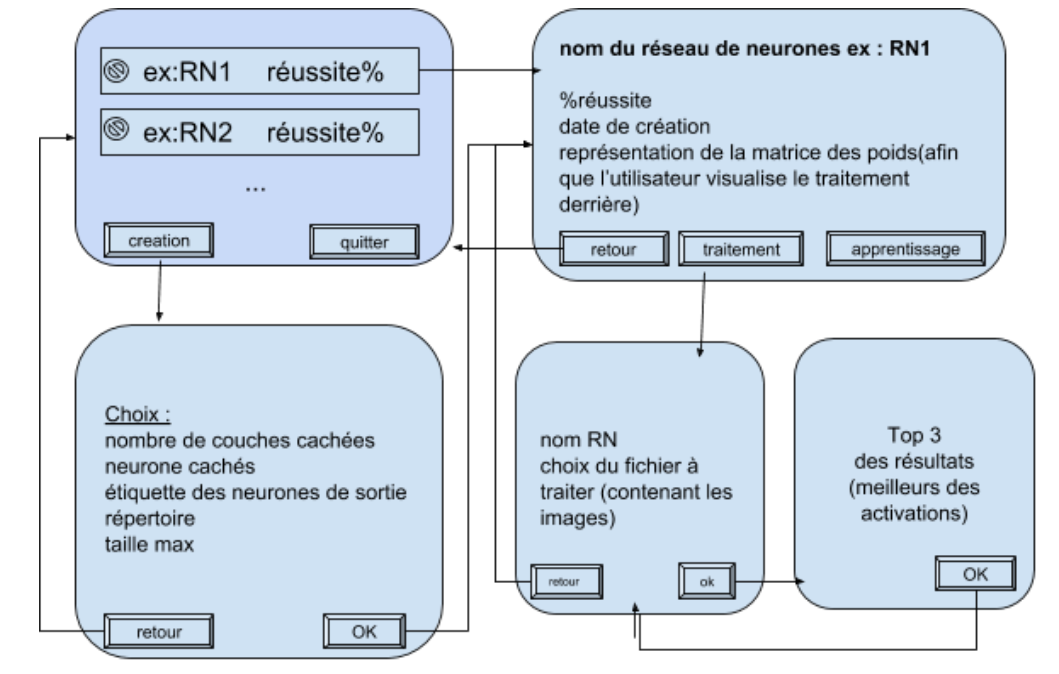
\includegraphics[height=244, width=400]{cap.PNG}
			\end{center}
		\subsection{Scénario de l'utilisation de l'interface}
	Lors de l'utilisation de l'application une page s'ouvre à l'utilisateur afin qu'il puisse faire ses manipulations. Il a un menu 
à sa portée où il peut selectionner des reseaux de neurones qu'il a déjà crée préalablement.
Il peut en choisir un et continuer l'usage de l'application ou bien il peut en créer un à nouveau en cliquant sur le bouton creer qui le dirigera vers une nouvelle page ou il devra remplir les differents champs avec les informations necessaires comme :\\ 
- tailleMax qui est la taille maximale des images qu'il devra analyser (qui precisera le nombre de neurones d'entrée du reseau de neurones).\\
- le nombre de couches cachées ainsi que le nombre de neurones.\\
- les etiquettes des neurones de sortie.\\
- choisir le repertoire d'image où elles sont stoquées.\\
 Ainsi il cliquera sur le bouton valider pour confirmer les informations, ou bien sur le bouton retour qui le redirigera à la page d'accueil.
Après validation des informations une nouvelle page s'ouvrira où l'utilisateur pourra lancer le traitement (c'est à dire la propagation). 
Là il devra choisir un fichier parmis d'autres pour fournir les images utiles au traitement.
Dans un premier temps, sans apprentissage, le résultat du traitement ne sera pas correct.
Le lancement de l'apprentissage du réseau de neurones permettera de lui apprendre à reconnaître des images. 
L'utilisateur pourra arrêter le processus d'apprentissage à n'importe quel moment ou le laisser continuer jusqu'à ce que le répertoire soit vide.
Après la fin de l'apprentissage l'utilisateur pourra tester son réseau de neurones en lui fournissant une image et pourra obtenir le top 3 des meilleurs activations des neurones de sortie du réseau. 
A la fin l'utilisateur pourra supprimer le réseau de neurones.
  
	\newpage

\section{Circulation d'informations entre les differents modules de l'application}
	\subsection{Organigramme et flux d'information}
		%illegal unit of mesure à verifier
		\begin{center} 
			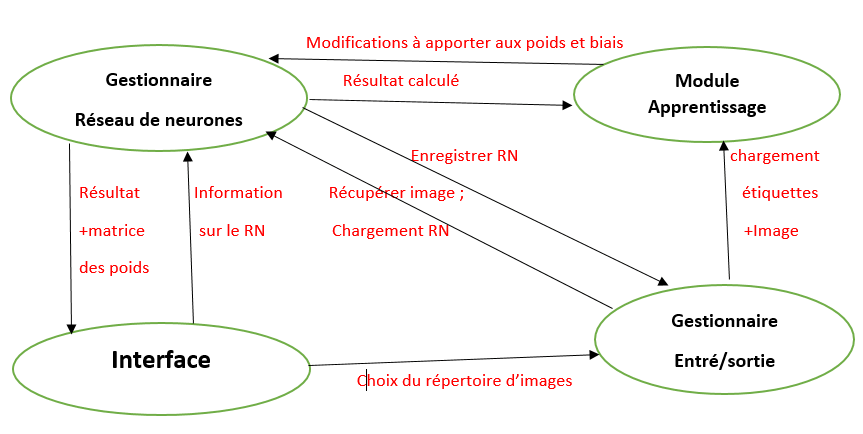
\includegraphics[height=244, width=300]{pic-min.PNG}
		\end{center}
			
	\subsection{Explication}	
	Dans l'interface l'utilisateur a la possibilité de choisir un réseau de neurones parmis d'autres qu'il a déjà crée.
Pour cela l'information sera transmise au gestionnaire du réseau de neurones afin qu'il puisse charger un réseau de neurones via la fonction chargerRN.
Il peut également créer un nouveau réseau de neurones, dans ce cas-là il devra entrer les données nécessaires pour sa création (la taille maximale, les couches d'entrées, les couches cachées ainsi que les étiquettes et le repertoire des images). 
Ces informations-là seront récupérées par le gestionnaire du réseau de neurones sous forme d'une structure appelée RN. 
On utilisera par la suite la structure dans la partie traitement(la propagation).
Dans cette partie, le réseau de neurones devra : \\
- récupérer une image du gestionnaire entrée/sortie à travers la structure Image.\\
- calculer le résultat et l'envoyer à nouveau à l'interface.\\
- envoyer la matrice des poids pour que l'utilisateur visualise au mieux les opérations qui s'effectuent derrière.\\
Le résultat calculé par le gestionnaire des réseaux de neurones sera récupéré via la fonction propagation par le module apprentissage pour pouvoir l'utiliser dans la retro-propagation.
Le module apprentissage va également récupérer les étiquettes ainsi que l'image du gestionnaire entrée/sortie via la fonction coupleImageEtiquette qui seront utile pour l'apprentissage.
Le module apprentissage récuperera aussi le top 3 des neurones de sortie via la fonction reconnaissance du gestionnaire réseau de neurones afin qu'on puisse calculer le nombre de reussite et d'échec en comparant la sortie obtenue avec celle attendue.
Par la suite les modifications à apporter aux poids et aux biais seront récupérées par le gestionnaire du réseau de neurones afin de les appliquer.
Le réseau de neurones sera par la suite enregistré dans le gestionnaire entrée/sortie à travers la fonction SaveRN.	

\section{Conclusion}
Pour conclure le choix du langage nous semble approprié pour la réalisation de notre application. En effet, nous n'avons pas rencontré de difficultés particulières lors de la rédaction du cahier des spécifications.
 Cependant, les operations sur les matrices et les vecteurs auraient pu être simplifiées. 
 Par exemple, le langage Python propose des fonctions effectuants des actions pénibles à implementer en langage C (commme la transposition des matrices).

\end{document}
